%ju 28-Mai-22 FM_U02_Leiterwiderstand_Loesung.tex
\section{Leiterwiderstand Übung 2}\label{leiterwiderstand-uebung-2}

\textbf{Aufgabe 1}

geg:

$l = 8,25~m$

$A = 0,75~mm^2$

$\rho = 0,0178~\frac{\Omega \cdot mm^2}{m} \,\text{(Kupfer)}$

ges: $R_l$

Formel

$R_l = \frac{p \cdot l}{A}$

Lösung

$R_l = 0,1958~\Omega$

\textbf{Aufgabe 2}

geg:

$R_l = 0,3648~m\Omega = 0,0003648~\Omega = \num{3,648e-04}~\Omega$

$\rho = 0,0178~\frac{\Omega \cdot mm^2}{m} \,\text{(Kupfer)}$

$d = 12,363~mm$

ges: $A, l$

Formel

$A = d^2 \cdot \pi$ oder $A = d^2 \cdot 0,785 \to (pi/4 = 0,785)$

$R_l = \frac{p \cdot l}{A} \to l = \frac{R_l \cdot A}{p}$

Lösung

$l = 2,459~m$

\textbf{Aufgabe 3}

geg:

$l = 4,5~m$

$R_l = 0,00267~\Omega = 2,666666~m\Omega = \num{2,67e-03}~\Omega$

$\rho = 0,0178~\frac{\Omega \cdot mm^2}{m} \,\text{(Kupfer)}$

ges: $A$

Formel

$R_l = \frac{p \cdot l}{A} \to A = \frac{p \cdot l}{R_l}$

Lösung

$A = 30,0~mm^2$

\textbf{Aufgabe 4}

\begin{figure}[!ht]% hier: !ht
\centering
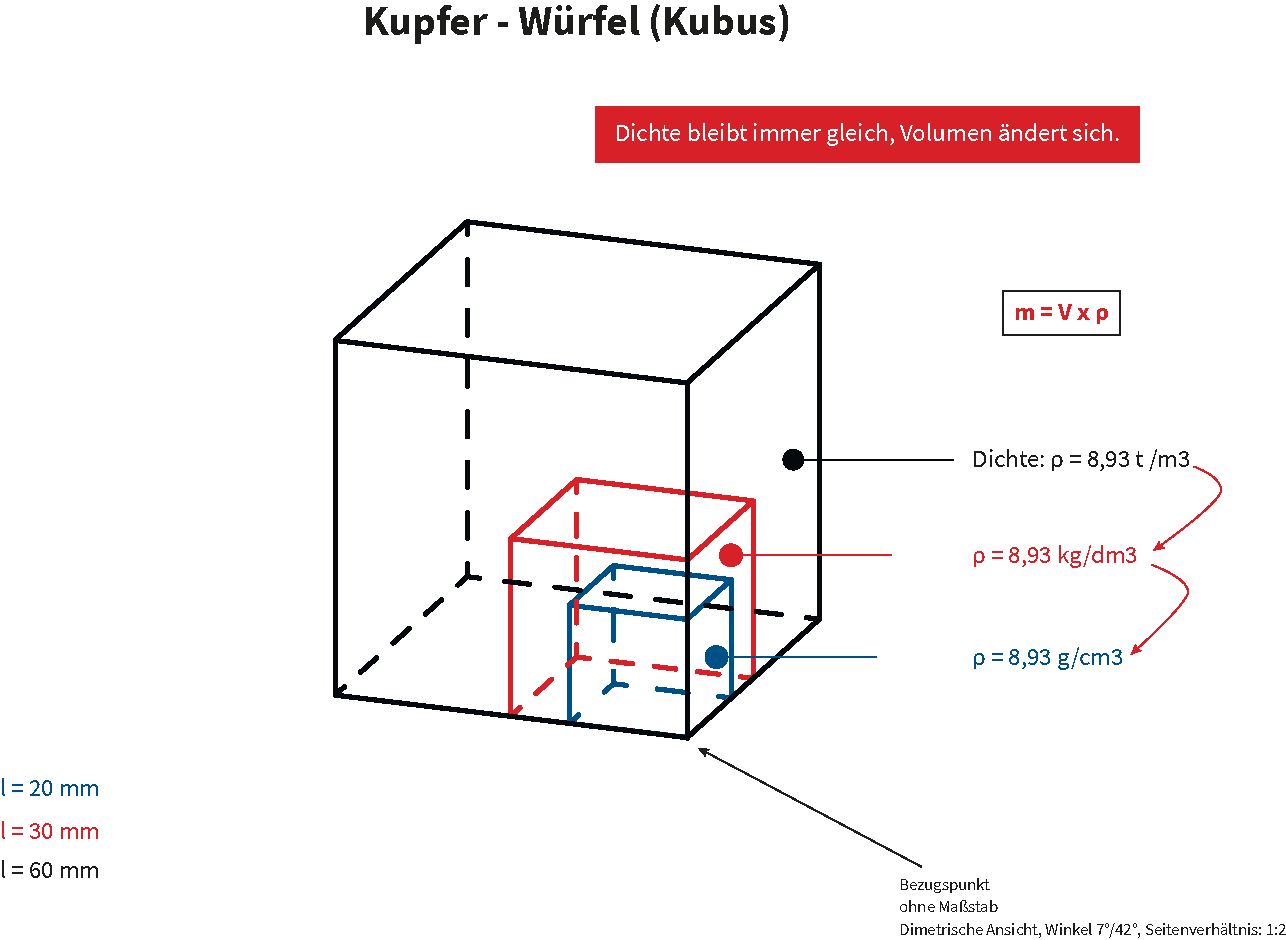
\includegraphics[width=0.6\textwidth]{images/Skizze/Kupfer_Wuerfel_Dichte.pdf}
\caption{Dichte / Volumen eines Kupferwürfels}
%\label{fig:}%% anpassen
\end{figure}

$\boxed{l = 2~cm}, V = (2~cm)^3 = 8~cm^3$

$m = 8~cm^3 \cdot 8,93~\frac{g}{cm^3} = 71~g$

$\boxed{l = 3~cm} = 0,3~dm, V = (0,3~dm)^3 = 0,027~dm^3$

$m = 0,027~dm^3 \cdot 8,93~\frac{kg}{dm^3} = 0,241~kg = 241~g$

$\boxed{l = 6~cm} = 0,06~m, V = (0,06~m)^3 = 0,000216~m^3$

$m = 0,000216~m^3 \cdot 8,93~\frac{t}{m^3} = 0,001929~t = 1929~g$

geg: Spule

$d_m = 36~mm = 3,6~cm$

$N = 1480$ (Windungen)

$d_D = 0,36~mm$

$p_{cu} = 8,93~\frac{t}{m^3}$ (Dichte)

$\rho = 0,0178~\frac{\Omega \cdot mm^2}{m} \,\text{(Kupfer)}$

ges: $A, l, R_l, G, V, m$

Formel

\emph{Kreisringfläche}: D = Außendurchmesser; d = Innendurchmesser; r =
Radius; $d_{mitte} = d_m$

$U = d \cdot \pi; \quad d_m = \frac{(D+d)}{2}; \quad r_m = \frac{(D+d)}{4}$

$A = \frac{d_D^2 \cdot \pi}{4}$

$l = U \cdot N \to l = \frac{d_m}{10} \cdot \pi \cdot N$

$R_l = \frac{\rho \cdot l}{100 \cdot A}$

$G = \frac{1}{R_l}$

$V = A \cdot h \to V = \frac{A}{100} \cdot l$

$m = V \cdot p_{cu}$

Lösung

$A = 0,1018~mm^2$

$l = 16738,4057~cm$

$R_l = 29,2711~\Omega$

$G = 0,0342~S$

$V = 17,0376~cm^3$

$m = 152,146~g$

\textbf{Aufgabe 5,1}

geg:

$R_l = 13,171999~m\Omega = 0,013171999~\Omega = \num{1,3171999e-2}~\Omega$

$\rho = 0,0178~\frac{\Omega \cdot mm^2}{m} \,\text{(Kupfer)}$

$d = 1,784576526~mm$

ges: $A, l$

Formel

$A = d^2 \cdot 0,785 \to (pi/4 = 0,785)$

$R_l = \frac{\rho \cdot l}{A} \to l = \frac{R_l \cdot A}{\rho}$

Lösung

$l = 1,85~m$

\textbf{Aufgabe 5,2}

Gleiche Leiterfläche für die Rückleitung, dass sie genauso hoch belastet
wird wie die positive Versorgungsleitung,

Sie liegen beide in Reihe, werden also vom gleichen Strom durchflossen,
